%!Tex Root = ../main.tex
% ./Packete.tex
% ./Design.tex
% ./Deklarationen.tex
% ./Vorbereitung.tex
% ./Aufgabe1.tex
% ./Aufgabe2.tex
% ./Aufgabe3.tex
% ./Aufgabe4.tex

\section{Appendix}

\setcounter{exercise}{1}

\begin{frame}{Appendix}{Unterschiede und Gemeinsamkeiten bei D-Latch und D-Flip-Flop}
  \begin{columns}
    \begin{column}{0.4\textwidth}
      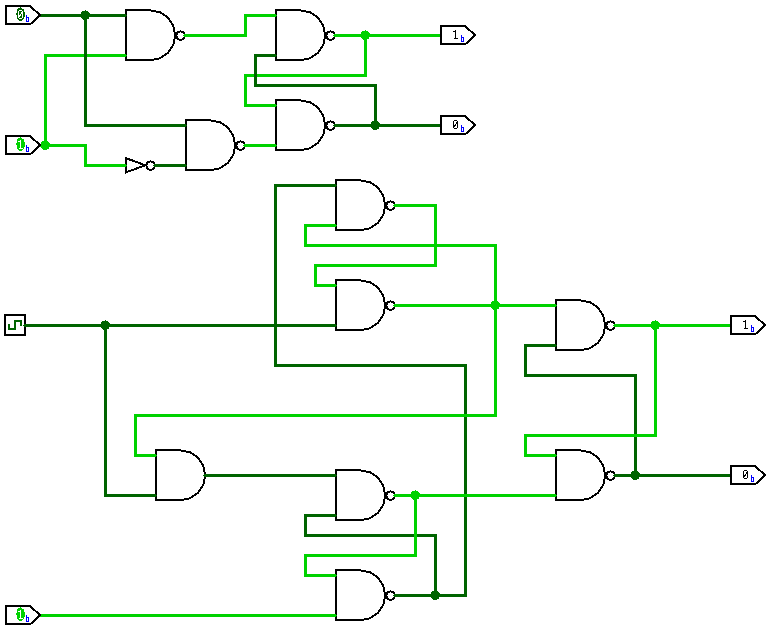
\includegraphics[width=0.6\paperheight, center]{./figures/011.png}
    \end{column}
    \begin{column}{0.6\textwidth}
      \begin{itemize}
        \item \alert{oberer RS-Flip-Flop} ist im \alert{Metastabilen Zustand} und hält dadurch den oberen Eingang des \alert{rechten RS-Flip-Flop} auf \alert{1}
        \item \alert{unterer RS-Flip-Flop} ist im \alert{Set Zustand} und hält dadurch den unteren Eingang des \alert{rechten RS-Flip-Flop} auf \alert{1}
        \item[\textcolor{PrimaryColor}{$\Rightarrow$}] \alert{rechter RS-Flip-Flop} ist dadurch im \alert{Wert-Speichern Zustand}
      \end{itemize}
    \end{column}
  \end{columns}
\end{frame}
\begin{frame}{Appendix}{Unterschiede und Gemeinsamkeiten bei D-Latch und D-Flip-Flop}
  \begin{columns}
    \begin{column}{0.4\textwidth}
      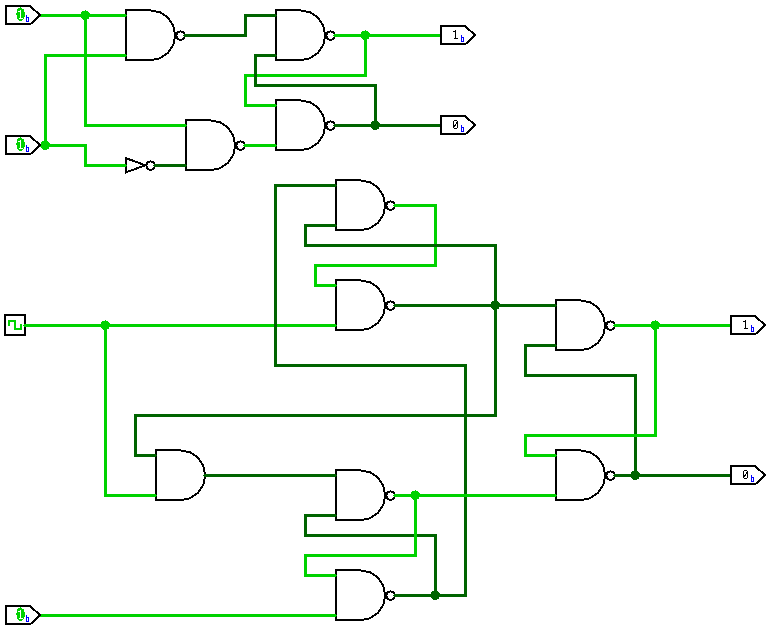
\includegraphics[width=0.6\paperheight, center]{./figures/111.png}
    \end{column}
    \begin{column}{0.6\textwidth}
      \begin{itemize}
        \item bei $d=1$
        \begin{itemize}
          \item \alert{oberer RS-Flip-Flop} geht bei \alert{clock} auf \alert{1} in den \alert{Set Zustand} über und hält dadurch den oberen Eingang des \alert{rechten RS-Flip-Flop} auf \alert{0}
          \item \alert{unterer RS-Flip-Flop} geht bei \alert{clock} auf \alert{1} in den \alert{Set Zustand} über und hält dadurch den unteren Eingang des \alert{rechten RS-Flip-Flop} auf \alert{1}
          \item[\textcolor{PrimaryColor}{$\Rightarrow$}] \alert{rechter RS-Flip-Flop} ist dadurch im \alert{Set Zustand}
        \end{itemize}
      \end{itemize}
    \end{column}
  \end{columns}
\end{frame}
\begin{frame}{Appendix}{Unterschiede und Gemeinsamkeiten bei D-Latch und D-Flip-Flop}
  \begin{columns}
    \begin{column}{0.4\textwidth}
      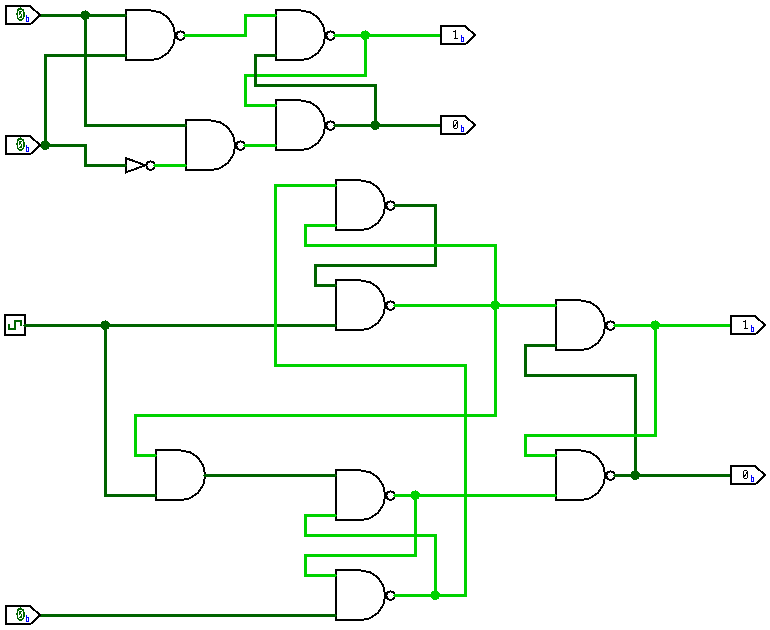
\includegraphics[width=0.6\paperheight, center]{./figures/001.png}
    \end{column}
    \begin{column}{0.6\textwidth}
      \begin{itemize}
        \item \alert{oberer RS-Flip-Flop} ist im \alert{Reset Zustand} und hält dadurch den oberen Eingang des \alert{rechten RS-Flip-Flop} auf \alert{1}
        \item \alert{unterer RS-Flip-Flop} ist im \alert{Metastabilen Zustand} und hält dadurch den unteren Eingang des \alert{rechten RS-Flip-Flop} auf \alert{1}
        \item[\textcolor{PrimaryColor}{$\Rightarrow$}] \alert{rechter RS-Flip-Flop} ist dadurch im \alert{Wert-Speichern Zustand}
      \end{itemize}
    \end{column}
  \end{columns}
\end{frame}
\begin{frame}{Appendix}{Unterschiede und Gemeinsamkeiten bei D-Latch und D-Flip-Flop}
  \begin{columns}
    \begin{column}{0.4\textwidth}
      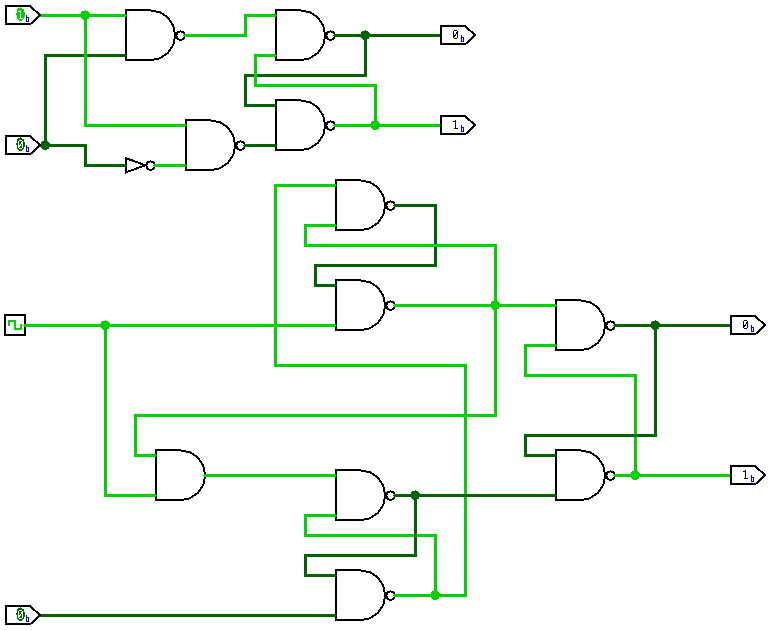
\includegraphics[width=0.6\paperheight, center]{./figures/100.png}
    \end{column}
    \begin{column}{0.6\textwidth}
      \begin{itemize}
        \item bei $d=0$
        \begin{itemize}
          \item \alert{oberer RS-Flip-Flop} geht bei \alert{clock} auf \alert{1} in den \alert{Wert-Speichern Zustand} über und hält dadurch den oberen Eingang des \alert{rechten RS-Flip-Flop} auf \alert{1}. Der \alert{obere RS-Flip-Flop} muss vorher in am unteren Eingang den Wert \alert{1} gehalten haben, da der obere RS-Flip-Flop wenn die Clock auf \alert{0} ist dafür sorgen muss, dass der \alert{rechte RS-Flip-Flop} im \alert{Wert-Speichern Zustand} ist, indem er eine \alert{1} hält
          
          \item \alert{unterer RS-Flip-Flop} geht bei \alert{clock} auf \alert{1} in den \alert{Reset Zustand} über und hält dadurch den unteren Eingang des \alert{rechten RS-Flip-Flop} auf \alert{0}
          \item[\textcolor{PrimaryColor}{$\Rightarrow$}] \alert{rechter RS-Flip-Flop} ist dadurch im \alert{Reset Zustand}
        \end{itemize}
      \end{itemize}
    \end{column}
  \end{columns}
\end{frame}
\begin{frame}{Appendix}{Unterschiede und Gemeinsamkeiten bei D-Latch und D-Flip-Flop}
  \begin{columns}
    \begin{column}{0.4\textwidth}
      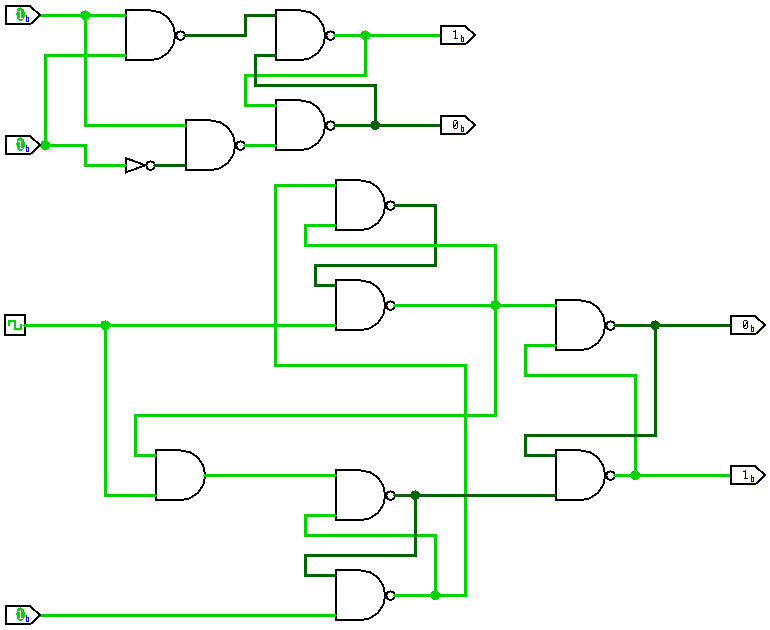
\includegraphics[width=0.6\paperheight, center]{./figures/11X.png}
    \end{column}
    \begin{column}{0.6\textwidth}
      % \setbeamertemplate{itemize/enumerate body begin}{\tiny}
      \begin{itemize}
        % \setbeamertemplate{itemize/enumerate subbody begin}{\tiny}
        \item der \alert{D-Flip-Flop} verhält sich gleich wie ein \alert{D-Latch} (siehe Aufgabe 4) allderdings mit dem \alert{Unterschied}, dass beim D-Flip-Flop der zu speichernde Wert in D beim Anheben der Clock von 0 auf 1 feststehen muss und im Nachhinein \alert{nicht geändert} werden kann solange die clock 1 ist und auch nicht während die Clock \alert{0} ist
        \begin{itemize}
          \only<1>{\item das wird erreicht indem die Werte an den beiden Eingängen des rechten RS-Flip-Flop durch den oberen und unterten RS-Flip-Flop gehalten werden wenn die Clock 1 ist 
          \item und indem der Wert 1 an einem der beiden Eingänge des rechten RS-Flip-Flop durch den oberen oder unteren RS-Flip-Flop passend gehalten wird wenn die Clock 0 ist}
          \only<2>{\item das Ändern von \alert{D} ändert die Zustände des oberen und underen RS-Flip-Flop zwar, aber niemals so, dass sich dadurch die an den Eingängen des rechten RS-Flip-Flop gehaltenen Werte ändern
          \item das Ändern von der \alert{Clock} kann nur einen der beiden Eingänge des rechten RS-Flip-Flop zwischen 0 und 1 wechseln lassen}
        \end{itemize}
      \end{itemize}
    \end{column}
  \end{columns}
\end{frame}
\begin{frame}{Appendix}{Unterschiede und Gemeinsamkeiten bei D-Latch und D-Flip-Flop}
  \begin{columns}
    \begin{column}{0.4\textwidth}
      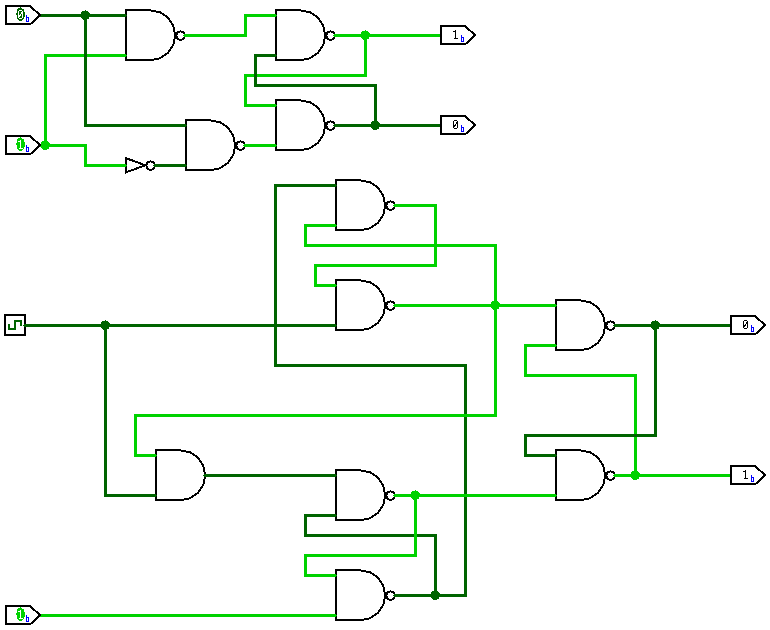
\includegraphics[width=0.6\paperheight, center]{./figures/01X.png}
    \end{column}
    \begin{column}{0.6\textwidth}
      \begin{itemize}
        \item beim D-Latch kann der gespeicherte Wert beliebig durch \alert{Ändern} des Wertes an D geändert werden solange die \alert{Clock 1} ist 
        \begin{itemize}
          \item nur während die \alert{Clock 0} ist wird der Wert gehalten und kann \alert{nicht geändert} werden
          \item damit der D-Latch sinnvoll verwendet werden kann müsste der Wert von D die \alert{ganze Zeit} über gehalten werden, während die Clock 1 ist + \alert{Setup-Zeit} und \alert{Hold-Zeit}, da jede Änderung während die \alert{Clock 1} ist den gespeicherten Wert ändern würde
        \end{itemize}
      \item beim D-Flip-Flop wird der gespeicherte Wert sowohl während die \alert{Clock 1 oder 0} ist gehalten und kann nur geändert werden, wenn die Clock von 0 auf high wechselt
      \begin{itemize}
        \item beim Wechsel der Clock auf 0 geht der \alert{rechte RS-Flip-Flop} in den Zustand \alert{Wert-Speichern} über
      \end{itemize}
      \end{itemize}
    \end{column}
  \end{columns}
\end{frame}
\begin{frame}{Appendix}{Unterschiede und Gemeinsamkeiten bei D-Latch und D-Flip-Flop}
  \begin{columns}
    \begin{column}{0.4\textwidth}
      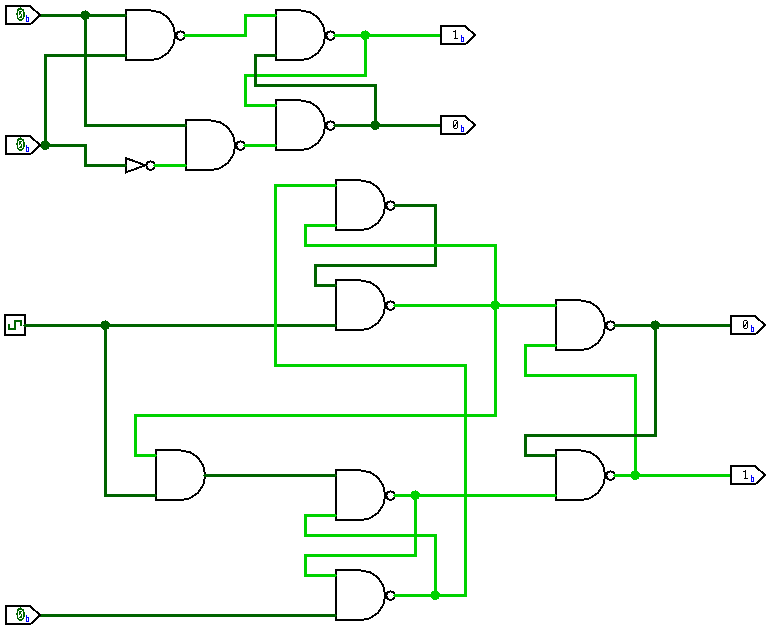
\includegraphics[width=0.6\paperheight, center]{./figures/00X.png}
    \end{column}
    \begin{column}{0.6\textwidth}
      \begin{itemize}
        \item \alert{D} sorgt dafür, dass der \alert{obere und untere RS-Flip-Flop} jeweils im \alert{\enquote{richtigen} Zustand} sind, so dass ein Flankenwechsel der Clock auf 1 den \alert{rechten RS-Flip-Flop} richtig einstellt 
      \end{itemize}
    \end{column}
  \end{columns}
\end{frame}
